\section*{27. Магнитное поле. Сила Ампера. Закон Био – Савара. Сила Лоренца.
Движение заряда в магнитном поле. Дрейф в скрещенных полях.}
 
\subsection*{Магнитное поле}

\imc[0.6\textwidth]{50.png}

Известно что между проводниками, по которым протекают электри-
ческие токи, возникают силы взаимодействия. Точно так же, как в элек-
тростатике, где введение электрического поля позволяет удобным обра-
зом описать взаимодействие статических зарядов, здесь полезно ввести
понятие \textit{магнитного поля}.

\textit{Магнитное поле в вакууме:}

\imc[0.4\textwidth]{55.png}

\[
d\vec{F_{12}}= \frac{I_1 I_2 }{c^2} \frac{[d\vec{l_2}\times [d\vec{l_1}\times \vec{r}]]}{r_{3}}  
\]

Постулируем, но понимаем, что: $dF_{12}\neq dF_{21}$

\subsection*{Сила Ампера и Закон Био – Савара}

\[
dF_{12}=\frac{I_2}{c}[d\vec{l}\times \vec{H}]-\textit{сила Ампера}  
\]

Где $\vec{H}:$

\[
dH=\frac{I}{c} \frac{[dl \times r]}{r^3} - \textit{закон Био-Савара}  
\]

\subsection*{Сила Лоренца}

\imc[0.4\textwidth]{56.png}

\textit{Сила Лоренца}-это сила, которая дейтвует на заряд со стороны магнтиного поля. 

\[
    dF_=\frac{I}{c}[d\vec{l}\times \vec{H}],\vec{j}=qn\vec{v}
\]

\[
Id\vec{l}=\vec{j}dV \Rightarrow Idl=jSdl
\]

\[
dF=\frac{1}{c}[Id\vec{l}\times \vec{H}]=\frac{1}{c}[\vec{j}dv \times \vec{H}]=\frac{1}{c} [dV\cdot nq\vec{v}\times \vec{H} ] \Rightarrow 
\]

\[
\Rightarrow\text{для единичного заряда: }\vec{F}=\frac{q}{c}[\vec{v}\times \vec{H}] 
\]

Если есть $\vec{H}\text{ и }\vec{E}\text{ , то: }\boxed{\vec{F}=q \bigg[\vec{E}+\frac{1}{c}[\vec{v} \times \vec{H}]\bigg] }$

\newpage

\subsection*{Движение заряда в магнитном поле}

\noindent
\begin{minipage}[c]{0.35\textwidth} % Левая часть: изображение
    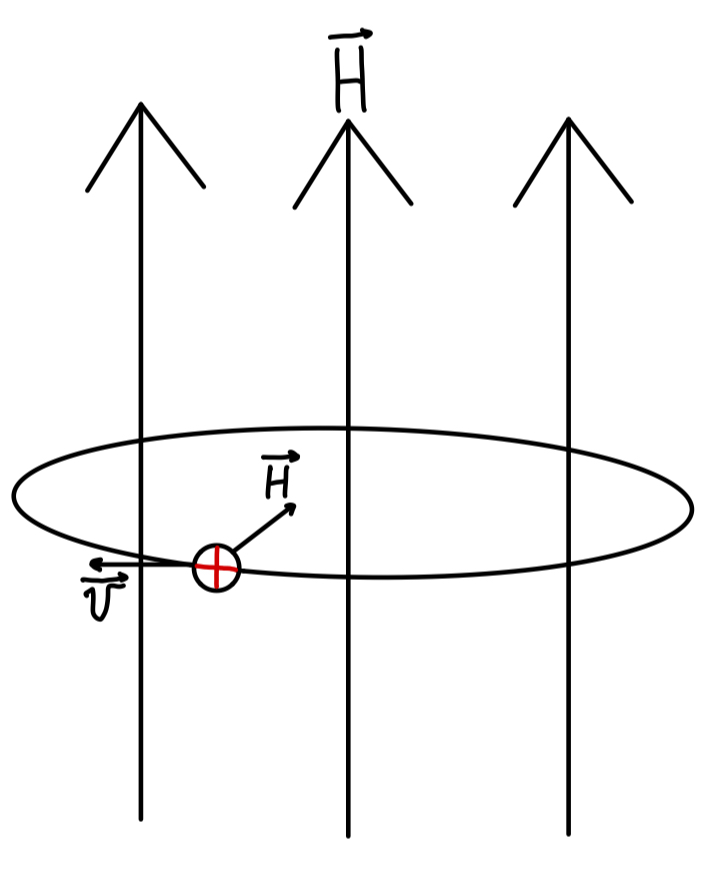
\includegraphics[width=\textwidth]{im/57.png}{\[\vec{v}\perp\vec{B} \]} % Ваше изображение
\end{minipage}%
\hfill
\begin{minipage}[c]{0.55\textwidth} % Правая часть: текст
    
    \[
    \vec{F}=\gamma m\dot{\vec{v}}=\frac{q}{c}[\vec{v}\times \vec{H}] \Rightarrow \dot{\vec{v}}=\left[ \left( -\frac{q\vec{H}}{\gamma mc}  \right) \times \vec{v} \right]
    \]
    \[
    \vec{\omega_c}=-\frac{q\vec{H}}{\gamma mc} 
    \]
\end{minipage}

\begin{figure}[h!]
    \centering
    % Первая картинка
    \begin{subfigure}{0.45\textwidth}
        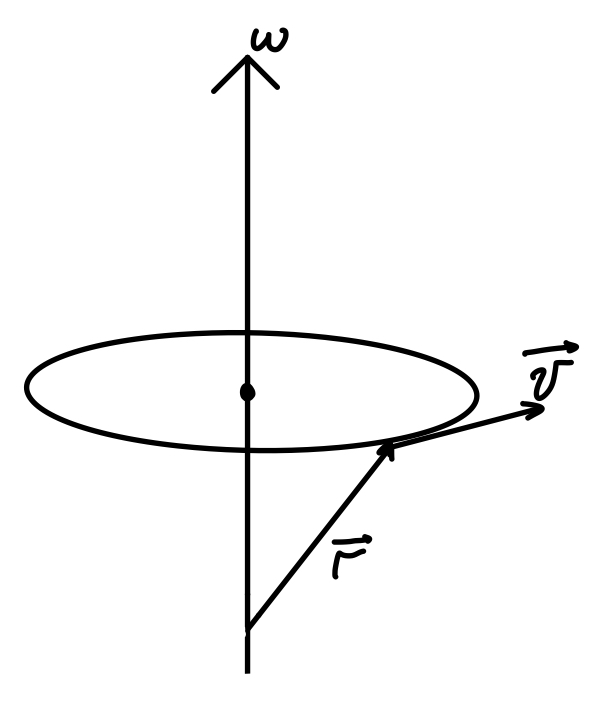
\includegraphics[width=\textwidth]{im/58.png} % Первая картинка
        \caption*{\(\vec{v}=\dot{\vec{r}}=[\vec{\omega}\times \vec{r}] \)}
        \label{fig:sub1}
    \end{subfigure}
    \hfill
    % Вторая картинка
    \begin{subfigure}{0.45\textwidth}
        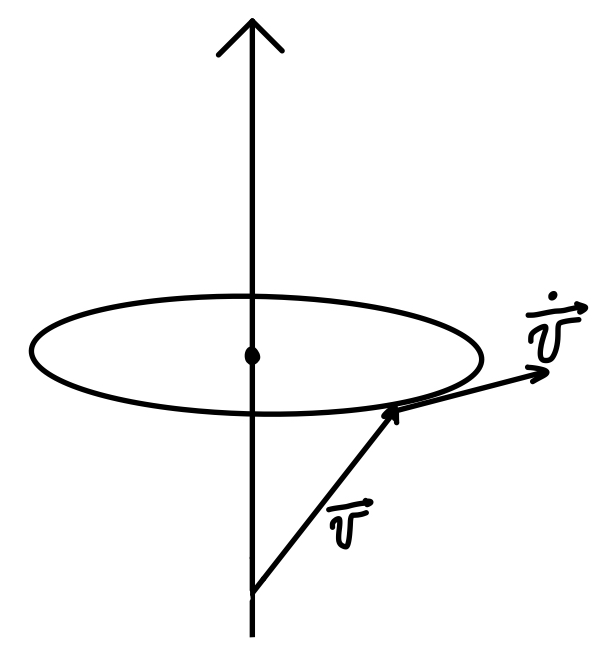
\includegraphics[width=\textwidth]{im/59.png} % Вторая картинка
        \caption*{\(\dot{\vec{v}}=[\vec{\omega_c}\times \vec{v}] \)}
        \label{fig:sub2}
    \end{subfigure}
    % Общая подпись для обеих картинок
    \caption*{}
    \label{fig:double}
\end{figure}

При малых скоростях:  $\omega_c= \frac{qH}{mc}.$

\[
\omega_c r=v_0 \Rightarrow r=\frac{v_0}{\omega_c} 
\]

\newpage

Неоднородное магнитное поле:

\imc[0.7\textwidth]{60.png}

В магнитном поле: $\vec{F}\perp\vec{v}\Rightarrow$ статичексое магнитное поле не совершает работу. 

\subsection*{Дрейф в скрещенных полях}

\imc[0.7\textwidth]{61.png}

\[
\vec{v}=\vec{\mathcal{U}}+\vec{\omega}
\]

Дрейфовая скорость, которая не зависит от $t -\vec{\omega}; $

Движение по окружнсоти + движение вдоль $\vec{H}$ с постоянной скоростью $ - \text{ }\vec{\mathcal{U} .}$

\[
m\dot{\vec{v}}=q\left( \vec{E}+\frac{q}{c}[\vec{v}\times \vec{H}]  \right)
\]

Пусть $\mathcal{U}$ есть решение уравнения без $\vec{E}: m\dot{\mathcal{U}}=\frac{q}{c}[\vec{v}\times\vec{H}]$

\[
\cancel{m\dot{\vec{\mathcal{U}}}}+m\dot{\vec{\omega}}=q\vec{E}+\cancel{\frac{q}{c}[\vec{\mathcal{U}}\times \vec{H}]}+\frac{q}{c}[\vec{\omega} \times \vec{H}] 
\]

Предпологаем, что $\vec{\omega}=\mathrm{const} \text{ и } \vec{\omega}\perp\vec{H}$, тогда $\dot{\vec{\omega}}=0:$

\[
q\vec{E}+\frac{q}{c}[\vec{\omega}\times \vec{H}]=0\Rightarrow[\vec{H}\times \vec{E}]+\frac{1}{c}[\vec{H}\times [\vec{\omega}\times \vec{H}]]=0  
\]

\[
c[\vec{H}\times \vec{E}]+\vec{\omega}H^2+H^2(\vec{\omega}\vec{H})=0\Rightarrow\boxed{\vec{\omega}=\frac{c[\vec{E}\times \vec{H}]}{H^2 }}\text{ } E<H
\]

Заряд движется вдоль эквипотенциали. 